\section{Die Komponenten}
\begin{frame}{Komponenten}{\target und \host}
 \begin{block}{\target}
  \begin{description}
   \item[Kernel] ein File
   \item[root] ein Filesystem
  \end{description}
 \end{block}
 \begin{block}{\host}
  \begin{description}
   \item[Toolchain] binutils, gcc
  \end{description}
 \end{block}
\end{frame}
\subsection{Target \target}

\begin{frame}{�bersicht}
 \begin{center}
  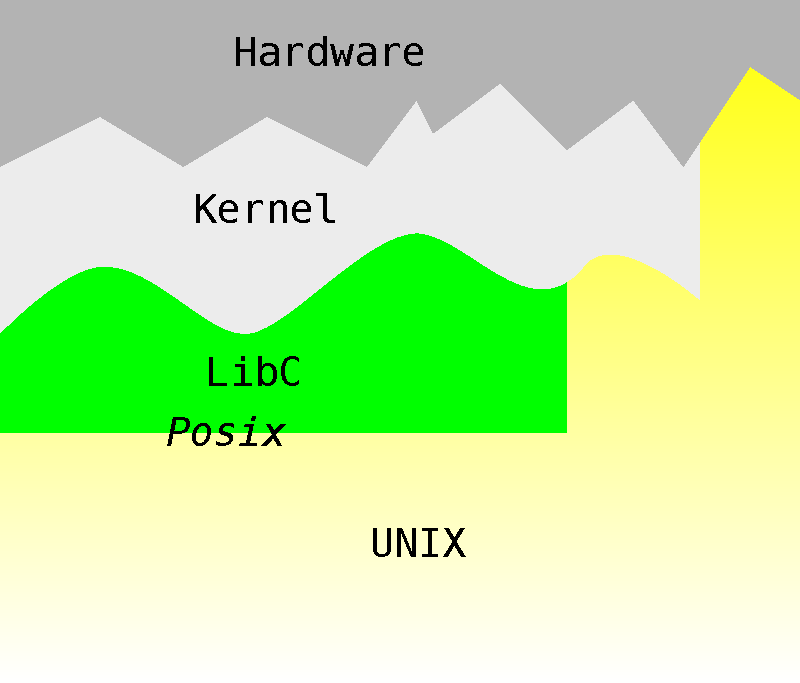
\includegraphics[width=8cm]{layers.pdf}
 \end{center}
\end{frame}

\begin{frame}{Die Komponenten}{f�r \target}
 \begin{description}
  \item[Hardware] \target
  \item[Kernel] zugeschnitten auf \target
  \begin{itemize}
    \item {\tiny \url{github.com/beagleboard/linux}}
  \end{itemize}	
  \item[root] das Filesystem
  \begin{description}
   \item[LibC] glibc 
   \begin{itemize}
    \item {\tiny \url{www.gnu.org/software/libc/index.html}}
   \end{itemize}	
   \item[\unix] busybox
   \begin{itemize}
    \item {\tiny \url{www.busybox.net/}}
   \end{itemize}
   \item[...] Weitere \unix basierte Komponenten
   \begin{itemize}
    \item das \cod{configure}, \cod{make}, \cod{make install} Triple 
   \end{itemize}
   \end{description}
 \end{description}
\end{frame}

\subsection{\host}
\begin{frame}{Toolchain}
 \begin{description}
  \item[binutils] linker \& Co.
  \item[gcc] compiler
  \begin{itemize}
   \item \cod{libgcc} die Bibliothek f�r den Compiler
  \end{itemize}
 \end{description}
 
 \begin{remarks}
 \item die Toolchain muss zweimal gebaut werden
 \begin{itemize}
  \item f�r den \kernel und \cod{libc} 
  \item f�r \unix/\posix
 \end{itemize}
 \item das target
 \begin{itemize} 
  \item \cod{cpu-vendor-os}
  
 \end{itemize}
 \end{remarks}
\end{frame}

\begin{frame}{Die Verzeichnisstruktur}
\dirtree{%
 .1 {\em somewhere\_on\_the\_host}.
 .2 tools.
 .3 common.h \DTcomment{used in (all) scripts}.
 .2 config \DTcomment{of the components}.
 .2 build \DTcomment{home of the build files}.
 .2 target-root \DTcomment{top of targer root}.
 .2 tc \DTcomment{the new toolchain}.
}
\end{frame}
